
\section{Programming Interface}
\label{sec:interface}
The target set of clients for our interface are higher-level language
compilers and runtimes such as Legion\cite{Legion12} as well as 
advanced systems programmers.  This class of clients expect total control
over the underlying hardware and transparent performance from an
implementation.  To support these demands we have designed our interface
to be as low-level as possible.  In many cases we have chosen to trade-off
ease of programmability for performance.  We eschewed any features that would
automatically be performed without being directed by the client.
Our goal in the design of this interface is to provide a set of low-level,
high-performance primitives that are asynchronous and composable.

Our interface organizes functionality into objects.  We describe
these objects in five parts: {\em events} for composing operations 
(Section~\ref{subsec:events}), {\em processors} for parallel computation 
(\ref{subsec:procs}), {\em deferred locks} for synchronization
(\ref{subsec:locks}), {\em physical regions} for data layout and movement
(\ref{subsec:phyreg}), and a {\em machine} object for introspection of the underlying
hardware (\ref{subsec:machmodel}).  In all cases (except for the
machine object which is a static singleton), instances of the objects
are light-weight {\em handles} that provide a unique name for an underlying
implementation.
Every handle is valid everywhere in the system, allowing handles to be freely copied,
passed as arguments to other tasks, or stored in the heap
without having to reason about the distributed nature of the system.
%%   Multiple copies of handles are permitted and handles can be 
%% passed by value.  Furthermore, every handle is valid everywhere in the system.  
%% This property allows a client to pass handles by value between computations 
%% without having to reason about the distributed nature of the system.
%We describe how we support this property in more detail in 
%Section~\ref{sec:impl}.

\lstset{
  captionpos=b,
  language=C++,
  basicstyle=\scriptsize,
  numbers=left,
  numberstyle=\tiny,
  columns=fullflexible,
  stepnumber=1,
  escapechar=\#,
  keepspaces=true,
  belowskip=-10pt,
  literate={<}{{$\langle$}}1 {>}{{$\rangle$}}1,
  %morekeywords={region,coloring,partition,spawn,disjoint,aliased},
  %deletekeywords=float,
}

\subsection{Events}
\label{subsec:events}
Events are the primary mechanism for describing dependences between operations in our system.
Listing~\ref{lst:eventapi} shows the interface for events.  An instance of the {\tt Event} type 
names a unique event in the system.  {\tt NO\_EVENT} (line 5) is a special instance
of an event that by definition has always triggered.  The event interface
supports testing whether an event has triggered (line 7) and waiting on
an event to trigger (line 9).  While these methods can be useful, the encouraged
use of events is passing them as preconditions for other operations.  The client can use the
{\tt merge\_events} call (lines 11-12) to create an event that triggers only when every
event in a given set of events has triggered.  An example using events follows in
Section~\ref{subsec:procs}.
%corresponding to the conjunction of a set of events.

In most cases events are created as the result of other
operations and the implementation is responsible for triggering these events.  Clients
can also create a {\tt UserEvent} (line 15) that is triggered explicitly by the client.

The common synchronization pattern in which multiple consumers are dependent on
a set of producers is supported by a {\tt Barrier} object, which is similar
to a user event, but does not trigger until the expected number of {\tt arrive}
operations have occurred.  To better support
composability and asynchronous operation, our interface differs from barriers in other programming
models\cite{MPI} in three fundamental ways:
%The common synchronization pattern in which multiple consumers are dependent on a 
%(potentially different) set of producers is supported by a {\tt Barrier} object,
%which is similar to a {\tt UserEvent}, but does not trigger until the expected
%number of {\tt arrive} operations have occurred.  Barrier constructs exist in other
%programming models\cite{MPI}, but in addition to the decoupling of the waiters from
%the arrivers, our barrier interface has two further improvements to better support
%composability and asynchronous operation:
\begin{itemize} \itemsep1pt \parskip0pt \parsep0pt
\item The set of producers of arrival calls can be different from the set of consumers waiting on the barrier.
\item An arrival operation can be made dependent on another event, allowing a client to
express that an operation should be completed before the barrier can trigger.
\item The expected arrival count of a barrier can be dynamically modified, allowing
barrier creation before needing to know the exact number of arrivals.
\end{itemize}

Both user events and barriers are a sub-type of events and can therefore
be used transparently to express dependences wherever events are used.
%Although user events and barriers are created and triggered differently,
%operations that express dependences on Events can transparently use
%UserEvents or Barriers as well.

%%   Users can also create another
%% type of event called a {\tt Barrier} that will require multiple arrivals before
%% the event is triggered.  The user can manage the number of arrivals that must
%% be seen as well as how many arrivals occur at a time.  Once a barrier's arrival
%% count goes to zero, the barrier will trigger.  Note that barriers in our interface
%% provide a superset of the functionality of traditional barriers since they can
%% be used in a blocking manner (via the {\tt wait} call), but are primarily used
%% asynchronously.  Lastly, since user events and barriers are sub-types of 
%% an event they can be used wherever an event is required.

\begin{lstlisting}[float={t},label={lst:eventapi},caption={Event Interface.}]
class Event {
  const unsigned id;
  const unsigned gen;
  static const Event NO_EVENT;
  // check if an event has triggered
  bool has_triggered() const;
  // wait on the event
  void wait() const;
  // Merge events together to create a new event
  static Event merge_events(Event ev1, Event ev2);
  static Event merge_events(const set<Event> &to_merge);
};

class UserEvent : public Event {
  static UserEvent create_user_event();
  void trigger() const;
};

class Barrier : public Event {
  static Barrier create_barrier(unsigned expected_arrivals);
  void alter_arrival_count(int delta) const;
  void arrive(unsigned count = 1,
                  Event wait_for = Event::NO_EVENT) const;
};
\end{lstlisting}

\subsection{Processors}
\label{subsec:procs}
Listing~\ref{lst:procapi} shows the interface for {\tt Processor} objects which allow for
the creation of parallel computations.  Processors provide a way of naming 
every computational unit in the machine.  We describe how to discover processor handles
in Section~\ref{subsec:machmodel}.  In the case of our current interface 
processors are either individual cores or discrete GPUs, but this is easily modified 
to include new processor types (line 10).   Processors support a single {\tt spawn}
method (lines 14-15) that launches a new {\em task} on that processor.
Note that because the spawn operation
is invoked on a processor handle, it is possible to launch a task on any
processor from anywhere in the system.  
The spawn call takes an optional event that must trigger before the task can begin.  
The spawn call returns an event that will trigger when the task completes.

Lines 18-24 of Listing~\ref{lst:procapi} show a simple example using 
the processor and event interface.  The {\tt diamond\_task} launches four
sub-tasks with a diamond dependence pattern, as shown in Figure~\ref{fig:procevents}.
The {\tt merge\_events} call
merges the events {\tt eb} and {\tt ec} to create the shared dependence
for the last sub-task.

\begin{lstlisting}[float={t},label={lst:procapi},caption={Processor Interface.},belowskip=0pt]
class Processor {
  const unsigned id;
  typedef unsigned TaskFuncID;
  typedef void (*TaskFuncPtr)
            (const void *args,size_t arglen,Processor p);
  typedef map<TaskFuncID, TaskFuncPtr> TaskIDTable;

  enum Kind {
    CPU_PROC,GPU_PROC,// ... future processor types
  };
  Kind kind() const;

  Event spawn(TaskFuncID func_id,const void *args,size_t arglen,
              Event wait_on = Event::NO_EVENT) const;
};
\end{lstlisting}

\begin{figure}
\begin{lrbox}{\mylistingbox}
\begin{lstlisting}
void diamond_task(const void *args,size_t arglen,Processor p){
  Event ea = p.spawn(TASK_A,NULL,0);
  Event eb = p.spawn(TASK_B,NULL,0,ea);
  Event ec = p.spawn(TASK_C,NULL,0,ea);
  Event em = Event::merge_events(eb,ec);
  Event ed = p.spawn(TASK_D,NULL,0,em);
}
\end{lstlisting}
\end{lrbox}
\subfigure{\usebox{\mylistingbox}}\\

\centering
\scalebox{0.8}{
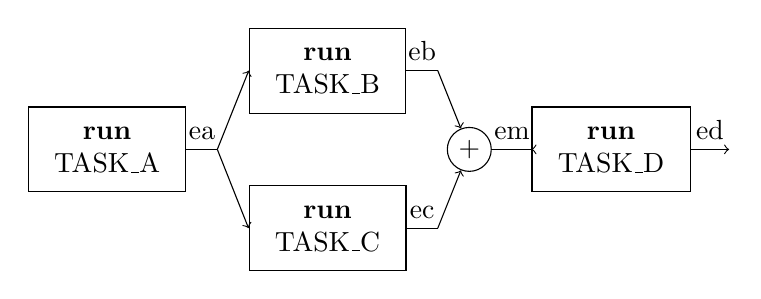
\begin{tikzpicture}
  %\path (1,3) node (t1) [shape=rectangle,draw] {run TASK\_A} -- node [right=1pt] {ea} +(0,-0.5) node[auto] {eax};
  \node (t1) at (0,0) [shape=rectangle,draw] {\begin{tabular}{c}{\bf run}\\TASK\_A\end{tabular}};
  \draw (t1) to node[auto] {ea} (1.4,0);

  \node (t2) at (2.8,1) [shape=rectangle,draw] {\begin{tabular}{c}{\bf run}\\TASK\_B\end{tabular}};
  \draw (t2) to node[auto] {eb} (4.2,1);
  \draw [->] (1.4,0) to (t2.west);

  \node (t3) at (2.8,-1) [shape=rectangle,draw] {\begin{tabular}{c}{\bf run}\\TASK\_C\end{tabular}};
  \draw (t3) to node[auto] {ec} (4.2,-1);
  \draw [->] (1.4,0) to (t3.west);

  \node (t4j) at (4.6,0) [shape=circle,inner sep=2pt,draw] {+};
  \draw (t4j) to node[auto] {em} (5.4,0);
  \draw [->] (4.2,1) to (t4j);
  \draw [->] (4.2,-1) to (t4j);

  \node (t4) at (6.4,0) [shape=rectangle,draw] {\begin{tabular}{c}{\bf run}\\TASK\_D\end{tabular}};
  \draw [->] (t4) to node[auto] {ed} (7.9,0);
  \draw [->] (5.4,0) to (t4.west);
  %
\end{tikzpicture}
}
%\vspace{-2mm}
\caption{Processor Example and Event Graph.\label{fig:procevents}}
\vspace{-4mm}
\end{figure}

\subsection{Deferred Locks}
\label{subsec:locks}

Events and barriers express ordering properties between operations, but 
%in many cases 
ordering is often too strict a requirement.  For many applications access to data need only be atomic and
not necessarily ordered.  Traditionally locks have been used to serialize access to
data.  However, all lock implementations that we are aware of require either blocking
or spinning, neither of which composes well with asynchronous operations.
{\em Deferred locks} are a new synchronization mechanism that allows for synchronization
in an completely asynchronous environment.  

\begin{lstlisting}[float={t},label={lst:lockapi},caption={Deferred Lock Interface.}]
class Lock {
  const unsigned id;
  Event lock(Event wait_on = Event::NO_EVENT) const;
  void unlock(Event wait_on = Event::NO_EVENT) const;
  // Create a new lock, destroy an existing lock
  static Lock create_lock(size_t payload_size = 0);
  void *payload_ptr();
  void destroy_lock();
};
\end{lstlisting}

\begin{figure}
\begin{lrbox}{\mylistingbox}
\begin{lstlisting}
void launcher_task(const void *args, size_t arglen, Processor p) {
  // Unpack lock, input events from arguments
  Lock needed = ...
  // Acquire lock, launch first subtask, release lock
  Event lock_event_1 = needed.lock(prev_event_1);
  Event task_event_1 = p.spawn(SUB, args_1, sizeof(args_1), lock_event_1);
  needed.unlock(task_event_1);
  // same for second subtask
  Event lock_event_2 = needed.lock(prev_event_2);
  Event task_event_2 = p.spawn(SUB, NULL, 0, lock_event_2);
  needed.unlock(task_event_2);
}
\end{lstlisting}
\end{lrbox}
\subfigure{\usebox{\mylistingbox}}\\

\centering
\scalebox{0.8}{
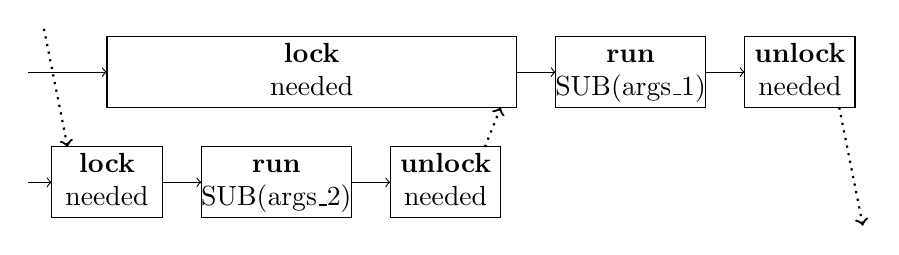
\begin{tikzpicture}
  \draw (1.0,1.5) rectangle (6.2,2.4);
  \node (l1) at (3.6,1.95) {\begin{tabular}{c}{\bf lock}\\needed\end{tabular}};

  \draw (6.7,1.5) rectangle (8.6,2.4);
  \node (t1) at (7.65,1.95) {\begin{tabular}{c}{\bf run}\\SUB(args\_1)\end{tabular}};

  \draw (9.1,1.5) rectangle (10.5,2.4);
  \node (u1) at (9.8,1.95) {\begin{tabular}{c}{\bf unlock}\\needed\end{tabular}};

  \draw [->] (0.0,1.95) to (1.0,1.95);
  \draw [->] (6.2,1.95) to (6.7,1.95);
  \draw [->] (8.6,1.95) to (9.1,1.95);

  \draw (0.3,0.1) rectangle (1.7,1.0);
  \node (l2) at (1.0,0.55) {\begin{tabular}{c}{\bf lock}\\needed\end{tabular}};

  \draw (2.2,0.1) rectangle (4.1,1.0);
  \node (t2) at (3.15,0.55) {\begin{tabular}{c}{\bf run}\\SUB(args\_2)\end{tabular}};

  \draw (4.6,0.1) rectangle (6.0,1.0);
  \node (u2) at (5.3,0.55) {\begin{tabular}{c}{\bf unlock}\\needed\end{tabular}};

  \draw [->] (0.0,0.55) to (0.3,0.55);
  \draw [->] (1.7,0.55) to (2.2,0.55);
  \draw [->] (4.1,0.55) to (4.6,0.55);

  \draw [->,dotted,thick] (0.2,2.5) to (0.5,1.0);
  \draw [->,dotted,thick] (5.8,1.0) to (6.0,1.5);
  \draw [->,dotted,thick] (10.3,1.5) to (10.6,0.0);

  %\path (1,3) node (t1) [shape=rectangle,draw] {run TASK\_A} -- node [right=1pt] {ea} +(0,-0.5) node[auto] {eax};
  %% \node (t1) at (0,0) [shape=rectangle,draw] {\begin{tabular}{c}{\bf lock}\\needed\end{tabular}};
  %% \draw (t1) to node[auto] {lock\_event} (2.4,0);

  %% \node (t2) at (3.2,0) [shape=rectangle,draw] {\begin{tabular}{c}{\bf run}\\SUB\end{tabular}};
  %% \draw (t2) to node[auto] {task\_event} (5.4,0);
  %% \draw [->] (2.4,0) to (t2.west);

  %% \node (t3) at (6.4,0) [shape=rectangle,draw] {\begin{tabular}{c}{\bf unlock}\\needed\end{tabular}};
  %% \draw [->] (5.4,0) to (t3.west);

  %% \draw [->,dotted,thick] (-1,1) to (t1.135);
  %% \draw [->,dotted,thick] (t3.45) to (7.4,1);
\end{tikzpicture}
}
%\vspace{-2mm}
\caption{Lock Example and Event Graph.\label{fig:lockevents}}
\vspace{-4mm}
\end{figure}

Listing~\ref{lst:lockapi} shows the 
interface for locks.  Unlike blocking locks, the {\tt lock} method (line 4) doesn't
block but instead always returns immediately with an event that will be triggered
when the lock has been acquired.  Just like the spawn method, the lock method also 
takes an optional event parameter as a precondition.  Similarly, the {\tt unlock} 
method (line 5) takes an optional event precondition parameter.

An important difference between deferred locks and blocking locks is that the processor
that requests the lock doesn't have to be the one that uses it.  A common
convention in writing code with deferred locks is to acquire locks on behalf of a task being
launched.  Listing~\ref{lst:lockapi} illustrates this with a simple example.  The
{\tt launcher\_task} is calling a sub-task that is going to require the {\tt needed}
lock.  A lock request is issued and the resulting {\tt lock\_event} is used as
a precondition for launching the {\tt SUB} task.  The unlock operation is then
made dependent
%precondition
on the event corresponding to {\tt SUB} task's completion.  The
{\tt SUB} task can run safely while holding the lock and the lock is released when the
{\tt SUB} task completes.  Figure~\ref{fig:lockevents} shows the event dependence graph, with
dotted lines representing a lock operation's dependence on a previous unlock.
Using deferred locks in this style prevents 
compute resources from waiting on locks by ensuring tasks only run when their needed
locks have already been acquired.

When a lock is used to mediate access to a piece of data, the first thing a task will usually
do after being granted the lock is access the data.  To be able to hide the latency of that
access as well, an additional feature of locks in our interface is the association of a lock with a
{\em payload}, a small (i.e. less than 4KB) 
piece of data that is moved around with the lock and guaranteed to be coherent while 
the lock is held.  The size of the payload is specified when the lock is created (line 7) and
the pointer to the local copy of the payload can be obtained from the {\tt payload\_ptr} method
(line 8).

Between deferred locks and barriers (described in Section~\ref{subsec:events}) clients 
have access to the same set of synchronization primitives that they have
in threading and bulk-synchronous interfaces.  However, these operations can now 
be composed with other asynchronous operations which is not possible in any other interface
of which we are aware.

%Deferred locks provide a super-set of the functionality of blocking locks.  As their
%name suggests, deferred locks can use the event corresponding to their lock acquire
%operation to defer execution until the lock acquire has been granted.  Deferred
%locks can also be converted back into a blocking lock by immediately waiting on the event
%returned from a call to {\tt lock}.  In addition, deffered locks also provide {\tt mode} and
%and {\tt exclusive} parameters that allow the user to specify whether other requests can acquire
%the lock simultaneously.  A lock can only be acquired in one mode at a time.  The
%{\tt exclusive} parameter specifies whether other owners are permitted once the
%current lock request is granted.


\subsection{Physical Regions}
\label{subsec:phyreg}
In distributed machines with discrete memories, data movement often consists of more
than a simple copy operation.  Many applications perform operations and transformations on
their data in conjunction with data movement for higher performance.  One common example is 
that applications accumulate reduction operations in a buffer and then, as part of a copy operation,
the reduction operations are applied to a destination buffer on the receiving side of the copy.  
To support these kinds of conjoined operations in an asynchronous environment, our interface 
must be aware of the structure of data so it can perform accompanying operations with 
data movement operations.  To describe the structure of data our interface uses {\em physical regions.}

A physical region is an allocation of data in a single memory in the memory hierarchy.  Physical
regions are grouped into {\em classes} which are sets of physical regions that share the
same names (i.e. addresses) for elements, but don't necessarily share the same data layout.  This
allows pointers to elements within regions to be used, even if the regions are copied from one memory
to another.  Our
interface supports sub-classing, but the details are omitted due to space constraints.  The
interface allows copies between any pair of physical regions that are of
the same class (or between super- and sub-classes).  

%Note, clients can still pass arbitrary arrays
%of bits via the processor {\tt spawn} call.

% Say something about dynamically modifying the number of elements in a class

\begin{lstlisting}[float={t},label={lst:regionapi},caption={Physical Region Interface and Example.}]
class Memory {
  const unsigned id;
  size_t size() const;
};

class RegionMetaData {
  const unsigned id;
  static const RegionMetaData NO_REGION;
  // Create and destroy metadatas
  static RegionMetaData create_region(size_t num_elmts, 
                                      size_t elmt_size);
  void destroy_region() const;
  // Create and destroy instances
  RegionInstance create_instance(Memory memory) const;
  void destroy_instance(RegionInstance instance) const;
  // Create a reduction-only instance
  RegionInstance create_instance(Memory memory, 
                        ReductionOpID redopid) const;
};

class RegionInstance {
  const unsigned id;
  static const RegionInstance NO_INST;
  // Copy between instances
  Event copy_to(RegionInstance target, 
                Event wait_on = Event::NO_EVENT);
  Event reduce_to(RegionInstance target, ReductionOpID redopid,
                Event wait_on = Event::NO_EVENT);
};
\end{lstlisting}

\begin{figure}
\begin{lrbox}{\mylistingbox}
\begin{lstlisting}
void reduction_ex(const void *args,size_t arglen,Processor p) {
  Memory m1,m2,m3; Processor p1,p2,p3;
  ... // Choose memory and processors, get redopid from args
  ReductionOpID redopid = ...;
  RegionMetaData meta = RegionMetaData::
                        create_region(num_elmts, elmt_size);
  Instance inst1 = meta.create_instance(m1, redop);
  Instance inst2 = meta.create_instance(m2, redop);
  Instance inst3 = meta.create_instance(m3);
  Event t1 = p1.spawn(REDUC, &inst1, sizeof(RegionInstance));
  Event t2 = p2.spawn(REDUC, &inst2, sizeof(RegionInstance));
  Event c1 = inst1.reduce_to(inst3, redopid, t1);
  Event c2 = inst2.reduce_to(inst3, redopid, t2);
  Event em = Event::merge_events(c1, c2);
  Event t3 = p3.spawn(USE, &inst3, sizeof(RegionInstance), em);
}
\end{lstlisting}
\end{lrbox}
\subfigure{\usebox{\mylistingbox}} \\

\subfigure{
\scalebox{0.8}{
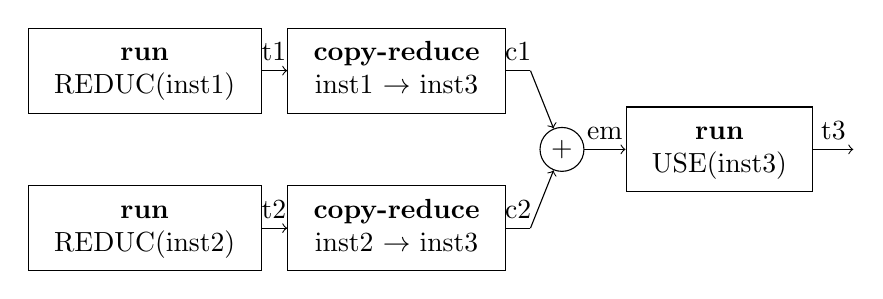
\begin{tikzpicture}
  %\path (1,3) node (t1) [shape=rectangle,draw] {run TASK\_A} -- node [right=1pt] {ea} +(0,-0.5) node[auto] {eax};
  \node (t1) at (0,1) [shape=rectangle,draw] {\begin{tabular}{c}{\bf run}\\REDUC(inst1)\end{tabular}};
  \draw (t1) to node[auto] {t1} (1.8,1);

  \node (t2) at (0,-1) [shape=rectangle,draw] {\begin{tabular}{c}{\bf run}\\REDUC(inst2)\end{tabular}};
  \draw (t2) to node[auto] {t2} (1.8,-1);

  \node (t3) at (3.2,1) [shape=rectangle,draw] {\begin{tabular}{c}{\bf copy-reduce}\\inst1 $\rightarrow$ inst3\end{tabular}};
  \draw (t3) to node[auto] {c1} (4.9,1);
  \draw [->] (1.8,1) to (t3.west);

  \node (t4) at (3.2,-1) [shape=rectangle,draw] {\begin{tabular}{c}{\bf copy-reduce}\\inst2 $\rightarrow$ inst3\end{tabular}};
  \draw (t4) to node[auto] {c2} (4.9,-1);
  \draw [->] (1.8,-1) to (t4.west);

  \node (t4j) at (5.3,0) [shape=circle,inner sep=2pt,draw] {+};
  \draw (t4j) to node[auto] {em} (6.1,0);
  \draw [->] (4.9,1) to (t4j);
  \draw [->] (4.9,-1) to (t4j);

  \node (t5) at (7.3,0) [shape=rectangle,draw] {\begin{tabular}{c}{\bf run}\\USE(inst3)\end{tabular}};
  \draw [->] (t5) to node[auto] {t3} (9,0);
  \draw [->] (6.1,0) to (t5.west);

\end{tikzpicture}
}
}
  %\vspace{-6mm}
  \caption{Reduction Example and Event Graph.\label{fig:reducevents}}
  \vspace{-4mm}
\end{figure}

Listing~\ref{lst:regionapi} shows a subset of the interface for physical regions.  
Each memory in the machine's memory hierarchy is named by a {\tt Memory} object (line 1).
The next object is a {\tt RegionMetaData} object (line 7), which defines a class of
regions.  Physical regions that belong to that class are created with the {\tt create\_instance}
method (line 16) and represented by {\tt RegionInstance} objects (line 23).  When creating a physical
region the client specifies the memory in which the physical region is going
to be allocated.  To maintain performance transparency, a new physical region can only be allocated
if the memory has sufficient capacity.
There is no automatic coherence of data between physical regions in the
same class.  It is the client's responsibility to manage data coherence using copies
between physical regions (line 28-29).  Like other operations copies can be
predicated on an event and return an event corresponding to completion.

If the only operations a task will perform on a region are reductions, a special reduction-only
instance can be created.  Rather than applying each reduction separately to the target instance,
the reduction operations can be accumulated in the reduction instance, and applied in bulk to 
the target using the {\em reduce\_to} operation.  This has several benefits.  First, it results
in much better performance, as we will show in section~\ref{subsec:reducmicro}), by reducing both
the total inter-node traffic and the overhead of that traffic while still allowing parallelism.
Second, a reduction-only instance is often smaller that the target instance, potentially improving
cache performance and helping address capacity issues for smaller memories (e.g. a GPU's device
memory).  For example, if reductions are being made to a single field in a larger structure, the 
reduction-only instance only needs to store that field and not the other fields that won't be 
modified by the reduction operation.

\texcomment{
If reductions are the only operations that will be performed on locations in a region instance,
a special reduction version can be created by providing the ID of a {\em reduction operator}
when the object is created (line 19).  Reduction-only region instances can 
increase the available parallelism and hide latency better, as we will show in 
section~\ref{subsec:reducmicro}.  The interface supports any reduction operation that
is commutative (i.e. multiple operations to the same location can be reordered without 
changing the final result) and is coded as an {\tt apply} method as shown on line 35.
Many commonly-used reduction operations are also {\em foldable} (e.g. $(l \text{ += } r_1) \text{ += } r_2$ can
be folded as $l \text{ += } r_1 + r_2$), and if the {\tt fold} operation and a {\em right identity}
(e.g. $0$ is a right identity for addition because $x + 0 = x$ for all $x$) are provided,
the runtime can use a {\em reduction fold instance}, described in section~\ref{subsec:reducimpl},
for even better performance.  Although the way they store data is very different,
reduction-only instances can be copied to other reduction-only instances (or normal 
instances) of the same class with the same asynchronous copy operations.  Copying between
instances with different layouts is only possible because physical regions provide 
the necessary information to understand the structure of the data.
}

%% Clients can also associate an operation as part of a physical region.  One example of
%% associating an operation with a physical region is shown on lines 13-14.  This instance
%% of the {\tt create\_instance} method
%% will create a physical region called a {\em reduction instance} that will be assoicated 
%% with the given {\tt ReductionOp} specified by the ID.  The interface for a {\tt ReductionOp} is shown on 
%% lines 26-33.  A reduction operation must have an {\tt apply} method, and can optionally 
%% implement two additional methods, {\tt init} and {\tt fold} that support additional 
%% optimizations described in Section~\ref{subsec:reducimpl}.  The two template parameters 
%% describe the base element type of the region ({\tt LHS}:left-hand-side) and the type of 
%% the argument to the reduction ({\tt RHS}:right-hand-side).  The reduction operation has 
%% total control over the choice of data layout for the reduction instance (not shown).
%% Reduction instances can be copied to other reduction instances with the same operation
%% or to regular physical regions of the same class.


An example using reduction-only regions is shown on lines 41-55 of Listing~\ref{lst:regionapi}.
Two reduction-only regions, {\tt inst1} and {\tt inst2}, are created in different memories to
be used with a reduction operation (lines 46-47).  (Reduction operations are registered at startup with integer IDs
as function pointers may not be portable across nodes.)  A physical region of the same class {\tt inst3}
is also created in a different memory (line 48).  Two tasks are launched that will apply
reductions locally into their respective reduction buffers (lines 49-50).  The resulting
events are then used to chain reduction copies back to {\tt inst3} after the tasks complete (lines 51-52).
The reduction operations accumulated in each of {\tt inst1} and {\tt inst2} are applied atomically
to {\tt inst3}.  The order in which the reduction operations are performed will be different from
the original order, but the requirement that reduction operations be commutative ensures the final
result is correct.  Finally, a merge on the events from the two reduction copies is 
performed and a final task using the results in {\tt inst3} is launched (lines 53-54).  This event
graph is shown in Figure~\ref{fig:reducevents}.

%% SJT - redundant with first paragraph in this subsection?
%% Reductions and reduction instances illustrate only a single case where physical regions provide 
%% the structure necessary to conjoin an operation with data movement.  Physcal regions make our
%% interface easily extensible to arbitrary transformations and operations as a part of data movment.
%% While physical regions are a slightly higher-level construct than an annonymous
%% buffer of bits, we believe that the optimizations they enable are important in an asynchronous
%% environment.  Clients also still have access to an interface for controlling data layout through
%% the operations associated with physical regions which mitigates the loss in generality.

%{\em Physical regions} are the mechanism for reasoning about
%the placement and movement of data in the interface.  Physical regions are an 
%allocation of data in a single memory in the memory hierarchy.  Listing~\ref{lst:regionapi} 
%shows a subset of the physical region interface.  The first object in the interface
%is a {\tt RegionMetaData} object (line 1).  Region meta-data objects provide the interface for the
%creation of sets of physical regions that possess the same number and type of elements (but not necessarily
%the same data layout).  The interface is only able
%to copy data between two physical regions that were created by the
%same region meta-data object.  A runtime error will be generated if a copy is attempted
%between two physical regions that were not created by the same meta-data object.

%An instance of a physical region is represented by a {\tt RegionInstance} object (line 17).
%When creating a physical region the programmer must specify the {\tt Memory}
%in which the physical region is going to be allocated (line 10).  Memories are described
%in more detail in Section~\ref{subsec:machmodel}.  Once the physical region is created it
%cannot be moved.   There is no coherence of data between physical regions created by the 
%same meta-data object.  It is the programmer's responsiblity to manage data coherence
%using copies between physical regions (line 22-23).  Just like other operations,
%copies can be predicated on an event and return an event corresponding to
%completion.  
%A copy between two physical regions can only be performed if copies
%are permitted between the two memories where the regions were created.  
%The legality of copies can be discovered using queries to the {\tt Machine} object
%described in Section~\ref{subsec:machmodel}.

%The data held inside a physical region is accessed by another kind of object called an
%{\em accessor} (not shown).  Accessors support read, write, and reduction operations
%to elements inside the physical region.  Accessors can be specialized for the case where
%all memory is known to be directly accessible to the executing processor, which allows 
%for direct references to elements.  In cases where not all memory is directly accessable, 
%accessors supply the level of indirection necessary to convert operations into remote 
%memory operations (RMAs) if supported by the underlying hardware.  
%An example of this is described in more detail in Section~\ref{sec:impl}.

%One special (but common) case for applications is when reductions need to be performed.
%For reductions it is usually more efficient to store reduction
%operations in a local reduction buffer and then merge reduction buffers together at a later
%point in time.  To support this case the interface allows for the creation of a special kind
%of physical instance called a {\em reduction instance}.  The call to {\tt create\_instance} on
%lines 13-14 takes a {\em reduction operation} to be associated with a physical instance which
%tells the interface to create a reduction instance.  Reduction instances can only be accessed
%using a reduction of the given reduction type; any other accesses will result in a runtime
%error.  A reduction operation is a functor which must have at least one method of the type
%$(T_1 \rightarrow T_2 \rightarrow T_1)$ which takes a region element of type $T_1$ and a value
%to be reduced of type $T_2$ and creates and new region element.  Reduction operations can optionally 
%support two additional methods: a method that supplies an initial value of type $T_2$ and a 
%fold method of type $(T_2 \rightarrow T_2 \rightarrow T_2)$.  The presence of these methods
%enable additional optimizations for reductions described in Section~\ref{subsec:reducimpl}.

%Reduction instances can be copied using the same interface as regular physical instances.
%It is only legal to copy a reduction instance to a regular physical instance or another
%reduction instance of the same reduction operator.  Any attempt to copy from a regular physical 
%instance to a reduction instance will result in a runtime error.  A copy from a reduction 
%instance to a regular physical instance will apply all the reductions in the reduction 
%buffer to the physical instance.  If a copy is from one reduction instance to another, 
%the two reduction buffers will be merged.  The semantics of a merge are dependent upon 
%the underlying implementation of reduction buffers which is discussed in more detail 
%in Section~\ref{subsec:reducimpl}.




\subsection{Machine}
\label{subsec:machmodel}
The last component of the interface is shown in Listing~\ref{lst:machineapi} and allows the
initialization and run-time introspection
of the current machine.
The {\tt Machine} object is a singleton object that the client creates at the start of a
program, providing a task table that maps task IDs to function pointers,
and then invoking the {\tt run} method (lines 9-10).
Any running task can get a pointer to the machine object with the
{\tt get\_machine} method (line 12) and use it to obtain lists of all the {\tt Memory} (line 13) or 
{\tt Processor} (line 14) handles in the system.  Using the affinity methods (lines 16-19),
the application can also determine which memories are accessible by each
processor and with what performance, as well as which pairs of memories support copy operations.
%are able to efficiently copy data between themselves.

%% in the machine.
%% Second, the machine object provides an interface for the client to 
%% discover properties of the underlying machine (lines 35-43).  The machine object maintains
%% sets of all the unique {\tt Processor} and {\tt Memory} handles in the system.  Processors
%% were described in Section~\ref{subsec:procs}.  For every memory in the system there also 
%% exists a {\tt Memory} handle with a unique ID.  Different memories often, but not always, 
%% imply a different address space.  Examples of different memories are described in
%% Section~\ref{sec:impl}.

%For
%example, in a large cluster each node would have a different {\tt Memory} handle
%corresponding to each node's DRAM memory.
%However, if the cluster supported multiple GPUs then there would be a different
%{\tt Memory} handle for each GPU's {\em zero-copy} memory which shares part of the 
%address space with the corresponding node memory.  Memories will be used for describing
%the placement of data described in Section~\ref{subsec:phyreg}.

%The machine interface 
%contains three different object types: {\tt Processor} (line 1), {\tt Memory} (line 17), and a 
%singleton {\tt Machine} object (line 22).  For every processor (i.e. CPU core or GPU) in 
%the system there exists a {\tt Processor} handle with a unique ID naming that processor.  
%{\tt Processor} objects support a single {\tt spawn} operation (line 13-14) that will
%launch a {\em task} on that processor.   

%% The machine object also maintains two relations between the set of processors
%% and the set of memories:
%% \begin{itemize}
%% \item Processor-Memory: for each processor-memory pair whether
%% the processor can directly access (read and write) the memory and 
%% latency and bandwidth properties if access is possible
%% \item Memory-Memory: for every pair of memories whether copies can be
%% performed and latency and bandwidth properties if copies are possible
%% \end{itemize}
%%
%% The client can query these two relations by the {\tt get\_*\_affinity} calls
%% (lines 40-43) to discover properties of the machine.  

%These calls populate a vector with affinity structures (not shown)
%that contain latency and bandwidth information.  The programmer can restrict the query
%by specifying a specific processor or memory, otherwise information is returned
%about all processors and memories in the system.  

\begin{lstlisting}[float={t},label={lst:machineapi},caption={Machine Interface.}]
class Machine {
  Machine(int *argc, char ***argv,
          const Processor::TaskIDTable &task_table);
  enum RunStyle {
    ONE_TASK_ONLY,ONE_TASK_PER_NODE,
    ONE_TASK_PER_PROCESSOR,
  };
  void run(Processor::TaskFuncID task_id = 0, 
        RunStyle = ONE_TASK_ONLY, const void *args, size_t arglen);

  static Machine* get_machine(void);
  const set<Memory>& get_all_memories(void) const;
  const set<Processor>& get_all_processors(void) const;

  int get_proc_mem_affinity(vector<ProcMemAffinity> &result,
          Processor restrict_proc = 0, Memory restrict_mem = 0);
  int get_mem_mem_affinity(vector<MemMemAffinity> &result,
          Memory restrict_mem1 = 0, Memory restrict_mem2 = 0);
};
\end{lstlisting}


